\chapter{Heterogeneous Cooperative Spectrum Sensing (CSS)}
\label{chapter3}

This chapter provides the background information needed to understand and implement cooperative spectrum sensing. It examines the basic outlines of a heterogeneous networks and how cooperative spectrum sensing (CSS) can help in enhancing the accuracy of signal source estimation. The fusion center (FC) collects the data from the sensor node network and processes it to make a reliable decision. Second, this chapter investigates various algorithms that can be used in heterogeneous network to estimate signal source. Finally, the necessary hardware and software tools used in the implementation of heterogeneous CSS prototypes is provided.

\section{Spectrum Sensing}
Spectrum sensing plays a key role in the decision-making part of cognitive radio networks. It is required by CR to detect the presence of spectrum white spaces and also to accurately estimate the presence of incumbent users (PUs). Since the PUs have  the prerogative on the spectrum band usage, so it is of paramount importance to avoid interfering with the PU when performing dynamic spectrum access. It is very challenging to get an accurate estimate under a practical fading environment based on conventional spectrum sensing techniques. Various non-idealities such as shadowing, multipath, and fluctuating noise variance can make it difficult to detect the primary user. In the case of fast  varying  channels over time, several works focus on improving the performance of the spectrum sensing and signal identification~\cite{hassan2012blind,kharbech2013blind,hassan2009automatic}. To combat the Doppler shift caused due to high-speed environments, algorithms~\cite{simon2013iterative} have been proposed for channel estimation and equalization. Cooperative spectrum sensing~\cite{ksgill} can be use to address many of these problems caused due to multipath, shadowing, and high Doppler shift. In the thesis, we evaluated the performance of cooperative spectrum sensing using soft and hard data fusion schemes via software-defined radio prototype hardware. The experiment confirmed that cooperation among sensor nodes will improve the spectrum sensing performance as a result of increased spatial-temporal diversity of the received signal source. The various types of spectrum sensing schemes are discussed below in the following subsections.

\subsection{Energy Detection}
In energy detection (ED) we use the energy spectra of the received signal and compare it against a predefined threshold level to estimate the presence of the signal.In an ED scheme we only rely on the energy of the signal in the frequency channel and no phase information is required. The key advantage of the ED scheme is that it does not require any prior information of the signal, \textit{i.e.}, type of modulation scheme, phase information or any other signal parameter. Energy detection can be considered as a binary hypothesis testing scheme and is given by~\cite{arhtn4}:

\begin{equation}
	\label{eq:1}
     y(n) = 
     \left\{
     \begin{aligned}
   &w(n),~~~~~~~~~\Hmat_0\\
   &s(n) + w(n),~\Hmat_1
    \end{aligned}
    \right.
\end{equation}
where $y(n)$ represents the received signal, $s(n)$ represents the signal source (PU), and $w(n)$ is the white Gaussian noise $w(n) \sim N(0,\sigma_n^2) $. $\Hmat_0$ describes the hypothesis when there is no signal present, while the hypothesis $\Hmat_1$ is the presence of signal. Figure~\ref{energydet} explains the energy detection scheme in the form of a block diagram. First, the analog signal $X(t)$ is converted into digital domain via analog-to-digital (ADC) converter, then the Fast Fourier Transform (FFT) block converts the signal from time domain to frequency domain. We then calculate the magnitude square of the signal and finally we take the average over the $N$ values to compute the decision statistic $\delta $. The $\delta$ is compared with the threshold to estimate the presence or absence of the signal.

\begin{figure}[ht!]
	\centering
	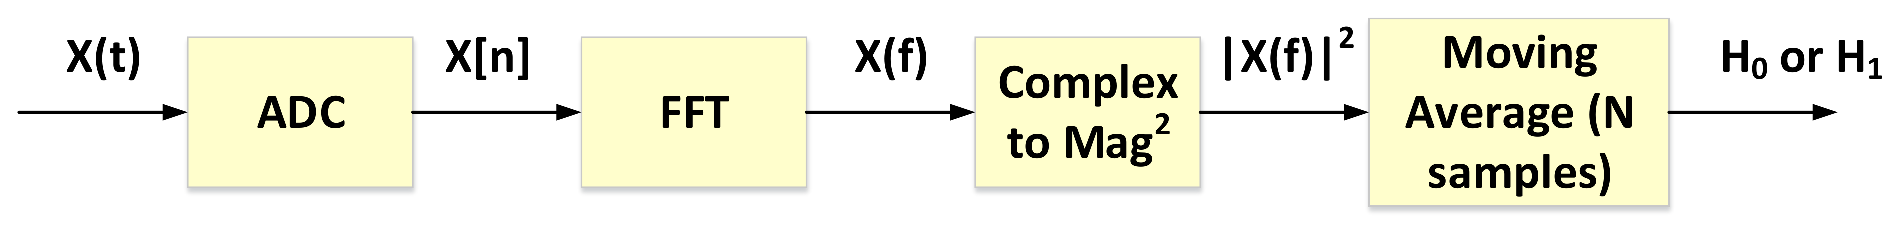
\includegraphics[width=\textwidth,keepaspectratio]{images/Gill/figs/energydet.eps}
    \caption{The block diagram describing the working of energy detection scheme~\cite{bookhtn1}.} 
\label{energydet}      
\end{figure}


The decision whether the signal is present or absent is decided by evaluating a local test statistic $L$ to see whether it is above or below certain fixed threshold $\tau$. 
The local test statistic $L$, which is the complex-magnitude squared of the FFT samples, is compared with $\tau$ using equation:

\begin{equation}
\label{eq:2}
	L = \sum_{n=1}^{M}{|y(n)|^2} = 
	\left\{
	\begin{aligned}
		<\tau,~\Hmat_0 \\
		>\tau,~\Hmat_1		
	\end{aligned}
	\right.
\end{equation}
where $|y(n)|^2$ is the energy of a specific FFT bin and $n~=~1,2,3...M$ are the number of samples received. The probability of false alarm $P_{fa}$ and probability of detection $P_d$ are given by~\cite{arhtn4}:
\begin{equation}
\label{eq:3}
P_f = Q\Bigg(\dfrac{\tau-M(2\sigma_n^2)}{\sqrt{M}(2\sigma_n^2)}\Bigg),
\end{equation}

\begin{equation}
\label{eq:4}
~~~~~~~P_d = Q\Bigg(\dfrac{\tau-M(2\sigma_n^2)(1+\gamma)}{\sqrt{M(1+2\gamma)}(2\sigma_n^2)}\Bigg).
\end{equation}
where $M_r$ is the number of samples used to estimate the power of the signal source in the node, $\sigma_{n,r}$ is the noise variance and $\tau$ is the threshold.

\subsection{Cyclostationary Method}

There are several applications where it is required to perform the modulation recognition and signal classification. Communication signals can be more accurately described as statistical processes which repeats themselves cyclically or periodically rather than a stationary process. Mathematically, Cyclostationary feature detection scheme can be described by the equation~\cite{bookhtn1}:

\begin{figure}[ht!]
	\centering
	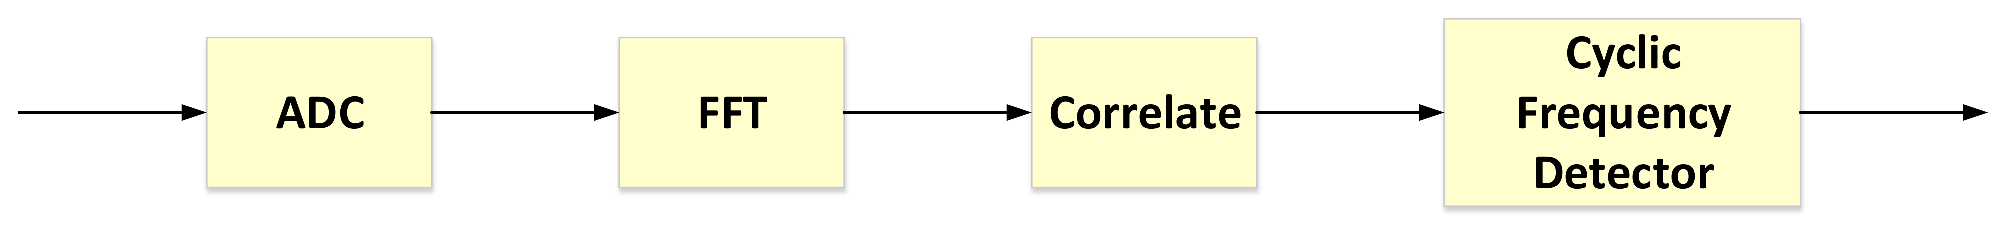
\includegraphics[width=\textwidth,keepaspectratio]{images/Gill/figs/cyclostationary.eps}
    \caption{The block diagram describing the working of cyclostationary feature detection scheme.} 
\label{cycl}      
\end{figure}

\begin{equation}
\label{eq:cyclo}
R_x(t,\tau) = E\Bigg\{x\bigg(t+\tau \bigg)x^*\bigg(t-\tau \bigg)\Bigg\} = \sum_{\{\alpha\}} R_x^{\alpha}(\tau)e^{j2\pi\alpha t}
\end{equation}
where $R_x$ is the cyclic autocorrelation function, $\alpha$ is the fundamental cyclic frequency.
The Eq.(\ref{eq:cyclo}) shows the autocorrelation of the observed signal $x(t)$ with periodicity $\tau$, $E\{.\}$ is the expectation operator, $\{\alpha\}$ is the set of Fourier components and $R_x^{\alpha}$ is the cyclic autocorrelation function (CAF) and is given by:

\begin{equation}
R_x^{\alpha} = \lim_{T\rightarrow \inf}\int_{-T/2}^{T/2} R_x(t,\tau)e^{-j2\pi\alpha t}.
\end{equation}

Figure~\ref{cycl} shows the block diagram implementation of cyclostationary feature detection scheme, where we correlate the frequency domain signal and then pass it to the cyclic frequency detection block and perform the signal classification.

\subsection{Matched Filter Detection}

In the matched filter detection method, a known signal is correlated with an unknown signal captured from the available radio resource to detect the presence of pattern in the unknown signal. It is an optimal filter that projects the received signal in the direction of the pilot signal $x_p$(n)~\cite{weidling2005framework}. The test statistic is given by:

\begin{equation}
T_{MD} = \sum_N y(n)x^*_p(n).
\end{equation}
where $y(n)$ is the received signal. The test statistic $T_{MD}$ is compared with a particular threshold to decide whether the signal is present or absent.The probability of detection $P_d$ and probability of false alarm $P_{fa}$ can be expressed as:
\begin{equation}
P_d = Q\bigg(\dfrac{\lambda-E}{\sqrt{E\sigma_{n,r}^2}}\bigg),
\end{equation}

\begin{equation}
P_{fa} = Q\bigg(\dfrac{\lambda}{\sqrt{E\sigma_{n,r}^2}}\bigg).
\end{equation}
where $E$ is the energy of the signal source, $\lambda$ is the detection threshold, and $\sigma_{n,r}$ is the noise variance. The use of matched filter is very limited due to the requirement of \textit{a priori} information which is not feasible in most cases. 

\section{Cognitive Radios}
Cognitive Radio (CR)~\cite{cogjm} is a communication systems paradigm that focuses on employing highly agile, environmentally aware, intelligent wireless platforms in
order to autonomously select and configure device operating parameters based on the prevailing radio and network environmental conditions~\cite{bookhtn1}. In general, cognitive radio may be expected to look at parameters, such as channel occupancy rate, available channels, bandwidth required for data transmission, and the modulation types that may be used. It must also look at the regulatory requirements set by the Federal Communications Commission (FCC). In some instances, a knowledge of geography and this may alter what we are permitted to do. Software-defined radios (SDRs) are mainly responsible for making cognitive radios used in wireless communications system a reality. Software radios provide the potential to personalize services, and they make the process of modifying the radio characteristics simpler. 

To facilitate the intelligent decision making capabilities in these cognitive radio systems, machine learning algorithms have been proposed in the literature~\cite{barker2008mission,haykin2005cognitive,newman2007cognitive,newman2008population} to automate the reconfiguration process. Figure~\ref{cograd} describes the various building blocks of a cognitive radio system. The spectrum sensing is performed to estimate the spectrum holes in the band and after the analysis the decision strategy is prepared. The radio is configured with the new parameters based on the radio environment and the spectrum decision made.  

\begin{figure}[ht!]
	\centering
	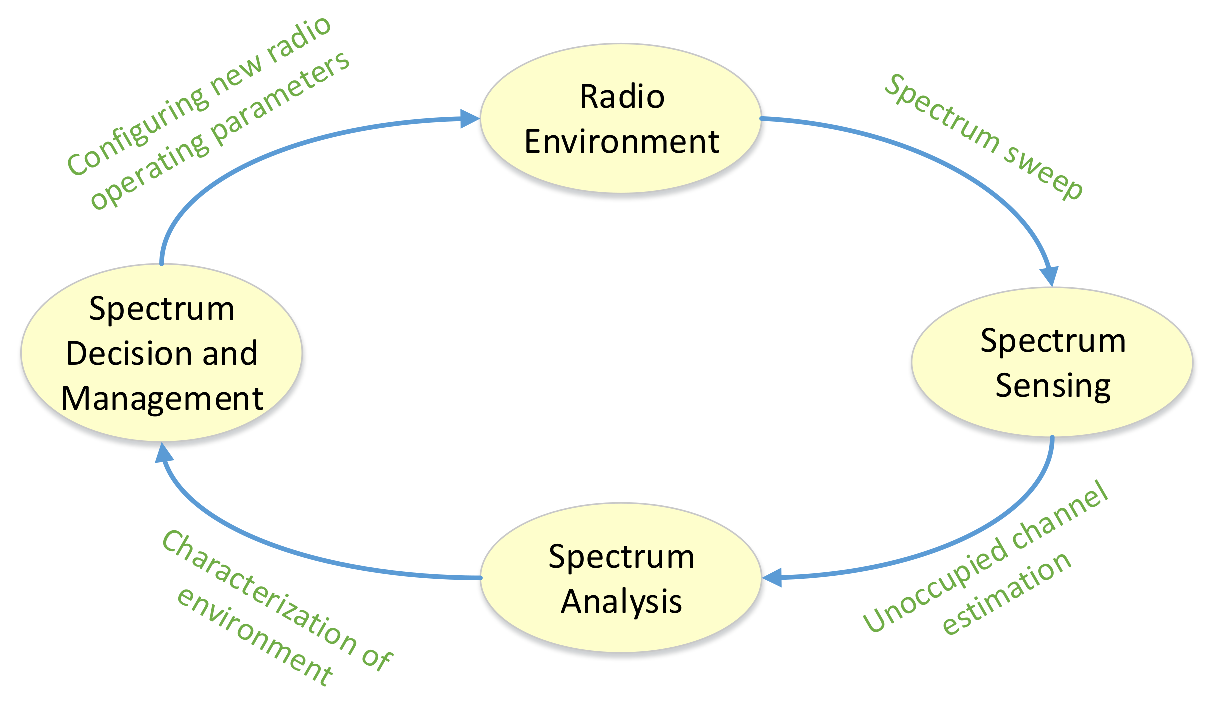
\includegraphics[width=\textwidth,keepaspectratio]{images/Gill/figs/cognitive_radio.eps}
    \caption{The block diagram explaining the basic parts of Cognitive Radio system. The operating parameters are configured based on the characterization of the wireless environment.} 
\label{cograd}      
\end{figure}

\section{CSS in Heterogeneous Networks}
In Heterogeneous CRNs, each radio is equipped with different numbers of antennas, sampling rates and RF characteristics. Additionally, each sensor node may experience distinct channel fading and suffer from different noise levels due to their respective locations and device performances, such as amplifiers and ADCs.  As a result, each node may have different sensing capabilities and reliability values. This is a universal and fundamental characteristic of a heterogeneous CRN, which requires robust algorithms to achieve high accuracy in signal source detection for estimating the presence of a primary user\cite{arhtn13}. In this thesis, we investigate the cooperative spectrum sensing in heterogeneous networks with a centralized FC, a transmitter acting as a signal source, and four sensor nodes. As explained earlier, we are using energy detection as one of the spectrum sensing technique since it possesses a very low implementation complexity~\cite{arhtn4}. The energy detection scheme detects the presence or absence of a signal source based on its intercepted energy signature. If the energy of the signal is higher than a certain threshold, this indicates that the channel is occupied. 


In cooperative spectrum sensing, each sensor node transmits the local sensing data to the fusion center for signal source detection. The local sensing data has to be quantized, thus yielding quantization errors. To minimize the quantization error in local test statistic $L$ and to reduce the effect of noise variance, the energy of the received signal $y(n)$ is normalized\cite{arhtn13}. The local test statistic $L$ for the $r^{th}$ sensor node is given as:
\begin{equation}
	\label{eq:5}
	L_r = \dfrac{1}{M_r\sigma_{n,r}^2}\sum_{r=1}^{M_r}|y(n)|^2
\end{equation}
where $M_r$ is the number of samples used to estimate the power of the signal source in the node,  $\sigma_{n,r}$ is the noise power variance.

In Eq.(\ref{eq:1}), $s(n)$ is considered to be a deterministic signal and $w(n)$ is a Gaussian random variable with a variance of $\sigma_n^2$. Based on CLT, $L_r$ will have a following distribution~\cite{inphtn7}:

\begin{equation}
	\label{eq:6}
	L_r = 
	\left\{
	\begin{aligned}
		& N(1,\dfrac{1}{M_r}),~~~~~~~~~~~~\Hmat_0 \\
		& N(\gamma_r+1,\dfrac{1+2\gamma_r}{M_r}),~\Hmat_1		
	\end{aligned}
	\right.
\end{equation}
where $\gamma_r$ is the received SNR of the $r^{th}$ SU. The local decision statistic $L_r$ is quantized before transmission due to the bandwidth constraint, and this can lead to quantization errors. The values of $L_r$ received by FC can be modeled as:
\begin{equation}
	\label{eq:7}
	 \beta_r = L_r + w_{q,r},
\end{equation}
where $\beta_r$ is the decision statistic received by the FC and $w_q$ is the noise added to the signal due to fading and quantization error. In \cite{arhtn14}, the $w_q$ is modeled as a Gaussian noise with zero mean and $\sigma_q^2$ variance.

\section{Software Defined Radios}
We have already explained about the cooperative spectrum sensing in heterogeneous networks, now in this section we will look at the platform for testing the CSS algorithms. The platform which we use is a new hardware frontier called Software-Defined Radio (SDR) and is discussed in details.

\begin{figure}[ht!]
	\centering
	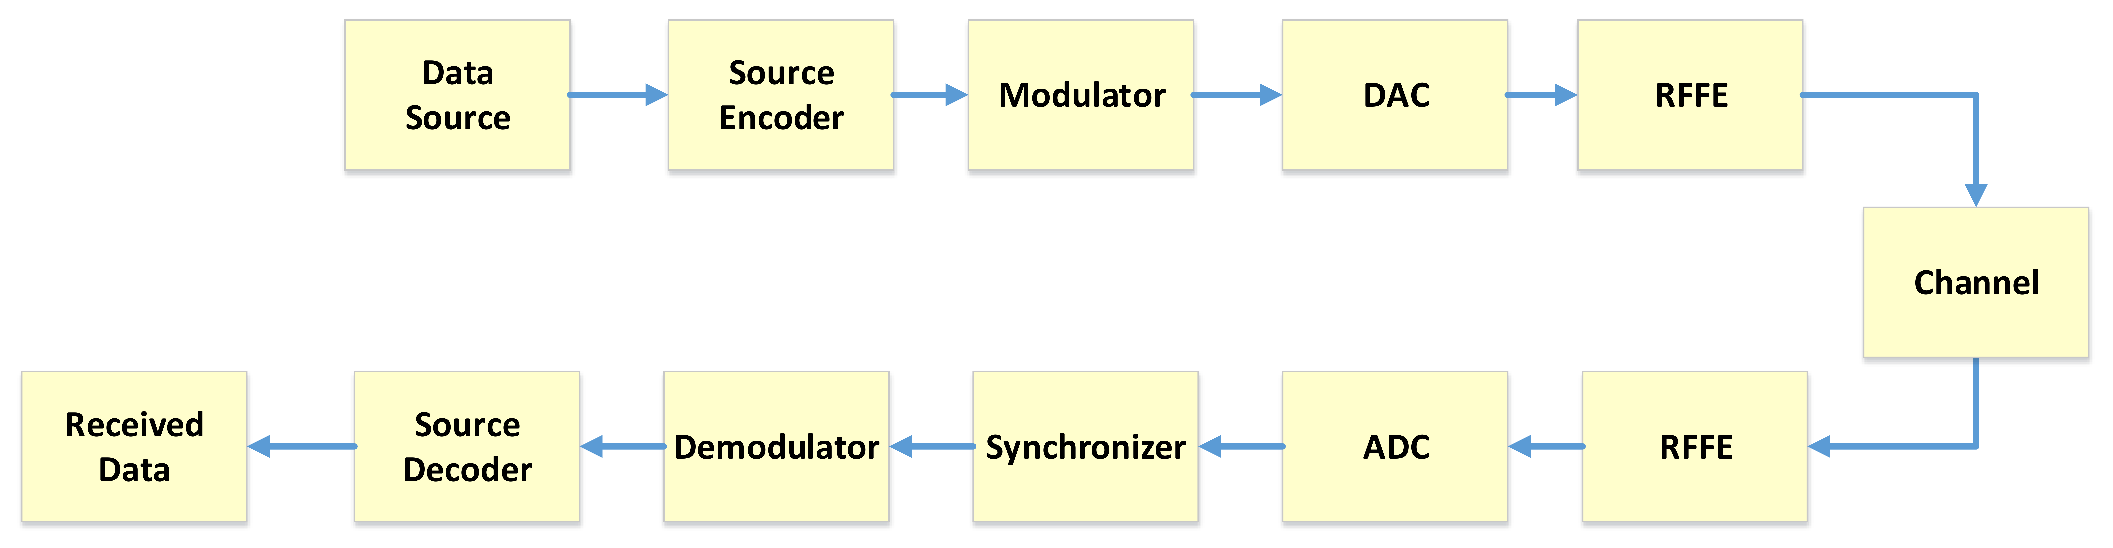
\includegraphics[width=\textwidth,keepaspectratio]{images/Gill/figs/softwaredefinedradio.eps}
    \caption{Software defined radio pushes all the adaptive elements and data manipulation operation into software. The goal of SDR is to provide or define all of the radio operation in software.} 
\label{sdr}      
\end{figure}

There has been a huge shift in the definition of a Software-Defined Radio and it has much to do with the question of where the hardware ends and the software begins. Mitola coined the term Software Defined Radio, which he described as a of digital signal processing (DSP) primitives, a meta-level system for combining the primitives into communication system (Tx, channel model, Rx, etc.), functions, and a set of target processors on which the software radio is hosted for real-time communications~\cite{267870}. Mitola explains in his thesis how software provides the flexibility which using hardware alone can never be achieved.

SDR technology existed since the 1970s~\cite{bookhtn1} but the key milestone in the advancement of SDR technology took place in early 1990s with the U.S. military initiative called SpeakEasy I/II. The SpeakEasy project was implemented to use programmable processing in order to emulate more than ten existing military radios, operating in frequency bands between 2 MHz and 2 GHz~\cite{392998}. With SpeakEasy, the operator could talk to ten radios operating under different standards with any hardware modifications. With all of these features, unfortunately, there were some shortcomings which left much to be desired. The device was large enough to fit on the back of a pickup truck~\cite{392998}, which is good for ground station but not if the mobility is an important factor. In 1992 the field programmable gate arrays (FPGA) were not computationally efficient, hence required a large amount of time to change their operating characteristics. 

The two software-defined radios we used in the thesis are Universal Software Radio Peripheral (USRP N210) and RTL-SDR R2832U. In the subsequent subsections, we discuss the two SDRs in detail.

\subsection{USRP N210 and RTL-SDR}
The USRP N210 and RTL-SDR are two very different SDR platforms when compared with each other, as shown in table~\ref{usrprtl}. The USRP N210 provides a very high bandwidth, dynamic range processing capability. The product architecture includes a Xilinx Spartan 3A-DSP 3400 FPGA~\cite{xilinx}, 100 MS/s dual ADC, 400 MS/s dual DAC, and gigabit ethernet connectivity to stream data to and from host processors. A modular design allows the USRP N210 to operate from DC to 6 GHz, while an expansion port allows multiple USRP N210 series devices to be synchronized and used in a MIMO configuration. An optional GPSDO module can also be used to discipline the USRP N210 reference clock to within 0.01 ppm of the worldwide GPS standard. The USRP N210 can stream up to 50 MS/s to and from host applications. Users can implement custom functions in the FPGA fabric, or in the on-board 32-bit RISC softcore. The USRP N210 provides a larger FPGA than the USRP N200 for applications demanding additional logic, memory and DSP resources. The FPGA also offers the potential to process up to 100 MS/s in both the transmit and receive directions. The FPGA firmware can be reloaded through the Gigabit Ethernet interface~\cite{usrp}.

\begin{table}[!ht]
\caption{Comparing different technical specifications of USRP N210 and RTL-SDR}
\centering
\begin{tabular}{| c | c | c |}
\toprule
Specifications  & USRP N210 & RTL-SDR \\ \hline
Maximum Sampling Rate  & 100 Msps  & 3.2 Msps\\ \hline
ADC Resolution  & 14 bits  & 8 bits\\ \hline
Frequency Range  & 400 MHz--4.4 GHz  & 24 MHz--1766 MHz\\
\bottomrule
\end{tabular}
\label{usrprtl}
\end{table}

\begin{figure*}[t!]
  \begin{center}
  \subfloat[\scriptsize RTL-SDR]{\label{fig:mapUrban}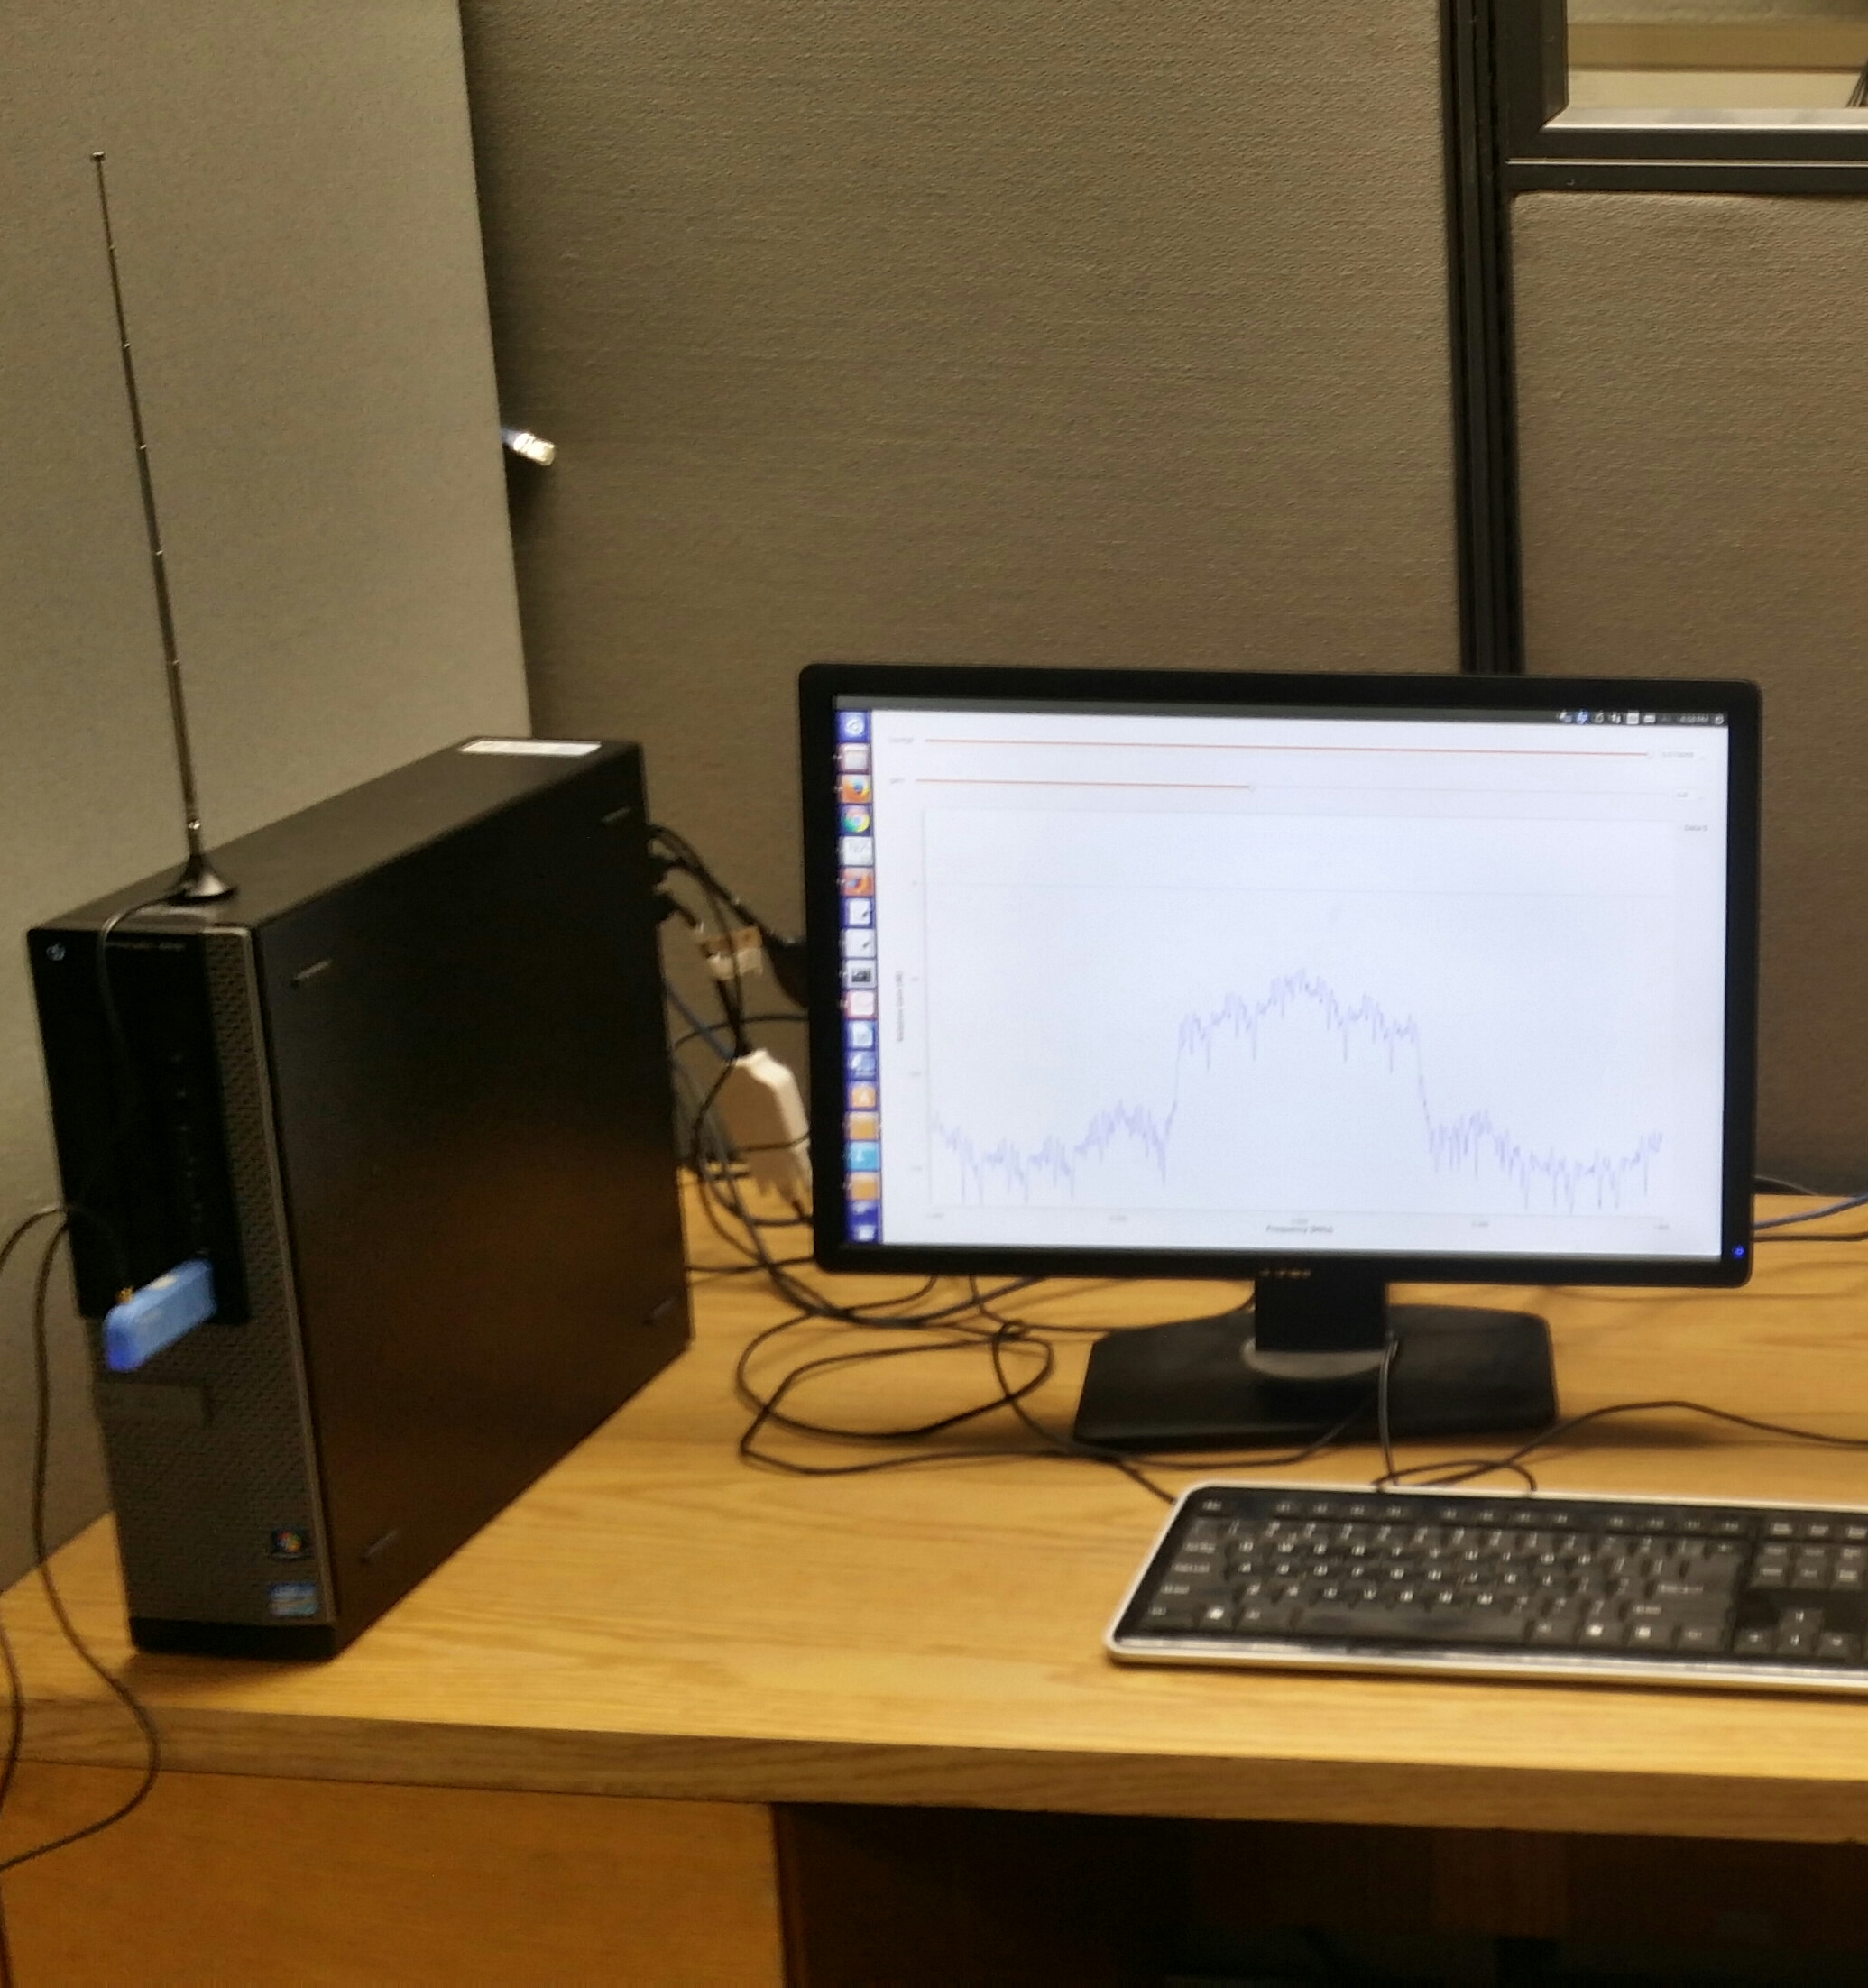
\includegraphics[width=0.45\textwidth]{images/Gill/figs/rtl.eps}}\hspace{1mm}
   \subfloat[\scriptsize USRP N210]{\label{fig:maphighway}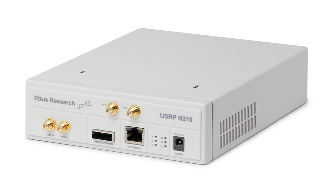
\includegraphics[width=0.45\textwidth]{images/Gill/figs/usrp.eps}}\hspace{1mm}
     \caption{RTL-SDR and USRP running a GNU Radio flow-graph and performing spectrum sensing at 450 MHz using normalized energy detection.} 
\label{usrprtl}      
   \end{center}
\end{figure*}

RTL-SDR is a very cheap software defined radio that uses a DVB-T TV tuner dongle based on the RTL2832U chipset. With the combined efforts of Antti Palosaari, Eric Fry, and Osmocom, it was found that the signal I/Q data could be accessed directly, which allowed the DVB-T TV tuner to be converted into a wideband software defined radio via a new software driver. Essentially, this means that a cheap \$20 TV tuner USB dongle with the RTL2832U chip can be used as a computer based radio scanner. This sort of scanner capability would have cost hundreds or even thousands of dollars just a few years ago. The RTL-SDR is also often referred to as RTL2832U, DVB-T SDR, RTL dongle or the “\$20 Software Defined Radio”. Figure~\ref{usrprtl} shows the RTL-SDR and USRP N210 running a GNU Radio flowgraph and performing spectrum sensing.

\subsection{GNU Radio and MATLAB}
We have used GNU Radio~\cite{gnradio} and MATLAB~\cite{matlab} software in the thesis to implement the cooperative spectrum sensing for hard decision and soft decision schemes. GNU Radio is an open source development toolkit that provides reconfigurable signal processing blocks to implement and test out software-defined radios and signal processing systems. GNU Radio allows for SDR developers to develop unique signal processing blocks and SDR systems. GNU Radio was started in 2001, originally forked from the SpectrumWare project developed at the Massachusetts Institute of Technology~\cite{Tennenhouse:1995:SSA:215530.215551}. Since 2001, the code base has undergone massive changes, containing almost no code from the original SpectrumWare project~\cite{bose1999virtual}. Physically the code consist of three languages Python, C++, and SWIG. Python provides the overarching control of the system or program, while C++ provides the actual signal processing blocks and mathematics. SWIG is a wrapper for C++ which allows Python to dynamically wrap around C++ and control or compile with it. Figure~\ref{gnuradio} better illustrates this architecture. It is also important to mention that there are significant paradigm shifts in the community, pushing more and more code to Python rather than C++, due to its easier programming syntax and structure~\cite{collins2013implementation}. In Figure~\ref{gnuradioflowgraph} we implemented a simple energy detection scheme by using available signal processing blocks in GNU Radio.

\begin{figure}[ht!]
	\centering
	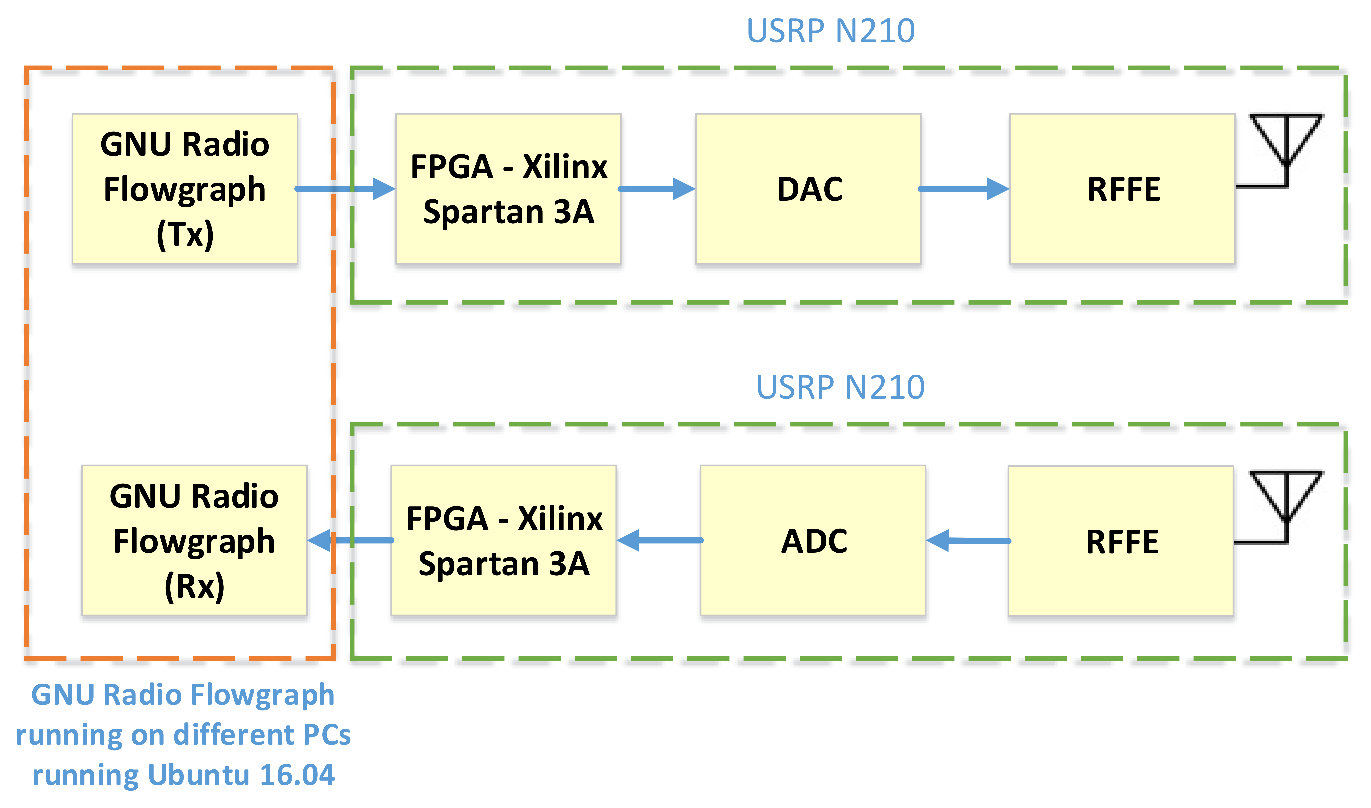
\includegraphics[width=\textwidth,keepaspectratio]{images/Gill/figs/gnuradio.eps}
    \caption{Block diagram describing the flow of information between GNU Radio and USRP N210. USRP N210 has in-built Xilinx Spartan 3A FPGA for designing reconfigurable SDR test-beds.} 
\label{gnuradio}      
\end{figure}

\begin{figure}[ht!]
	\centering
	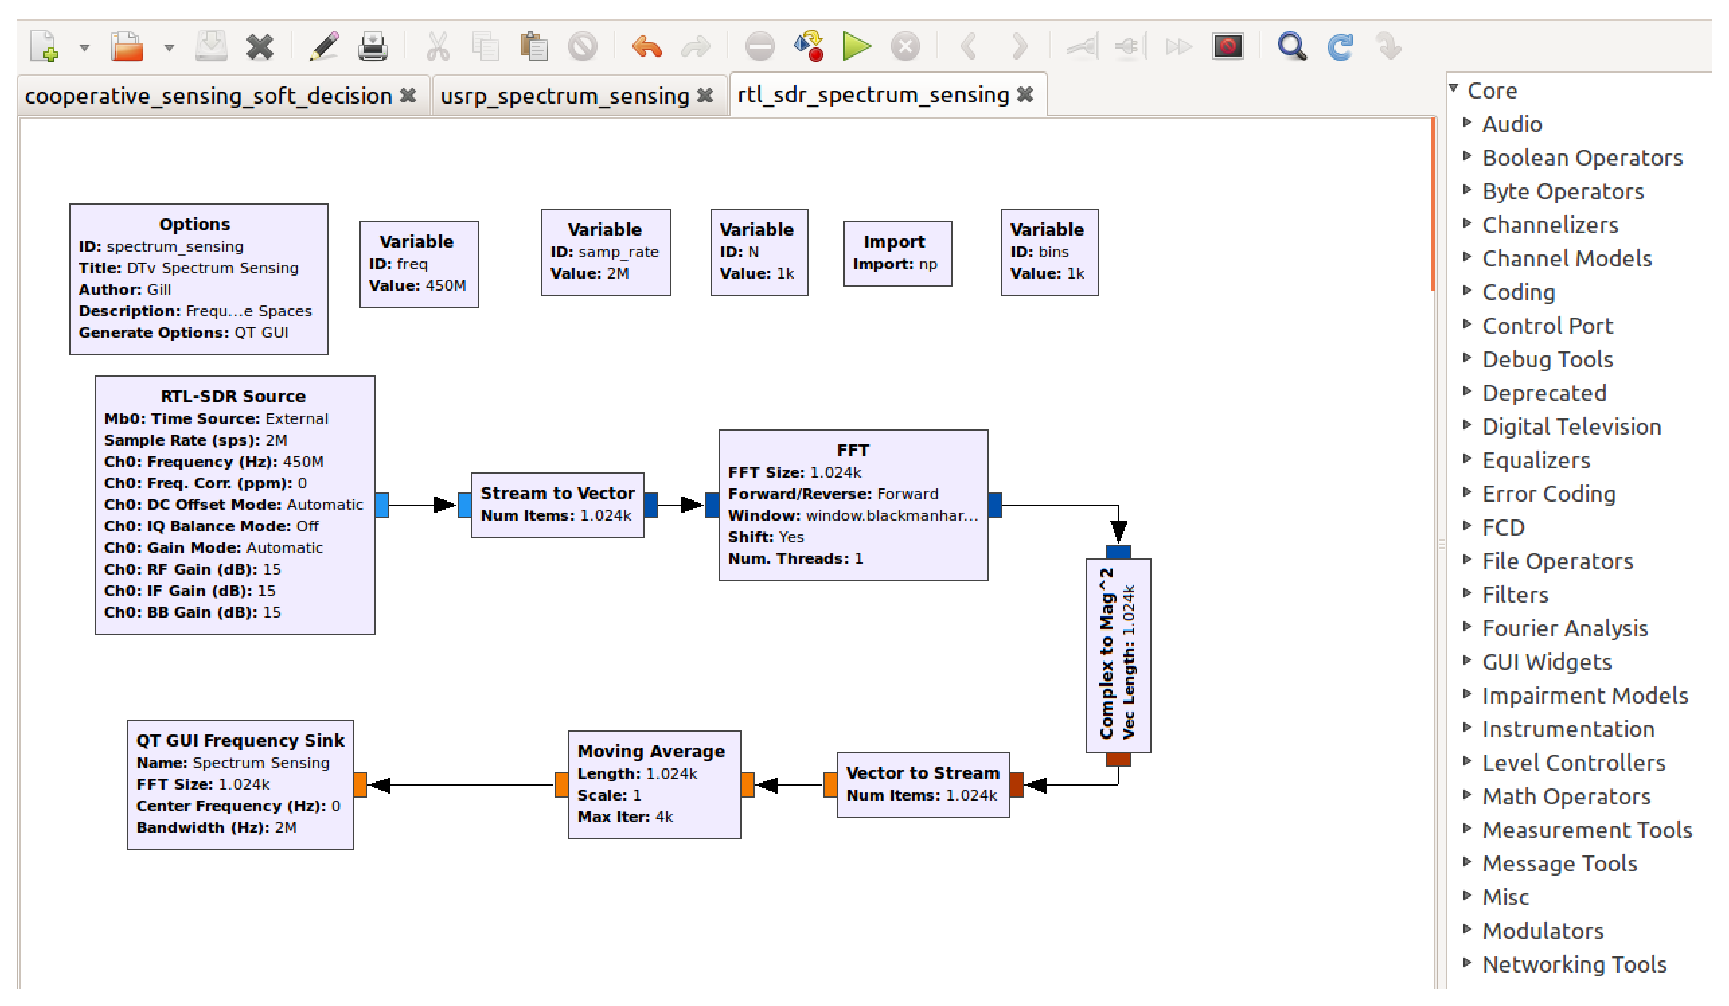
\includegraphics[width=\textwidth,keepaspectratio]{images/Gill/figs/gnuflowgraph.eps}
    \caption{GNU Radio flow-graph for spectrum sensing using energy detection using RTL-SDR source.}
\label{gnuradioflowgraph}      
\end{figure}

The GNU Radio software provides the framework and tools to build and run software radio or just perform general signal processing applications. The GNU Radio applications themselves are generally known as ''flow-graphs'', which are a series of signal processing blocks connected together, thus describing a data flow. GNU Radio provides a very structured framework of flow design. Data processing segments are highly self contained in order to minimize error propagation during system debugging. Since the software is open-source, full access to all code is provide, giving low-level access to all operations within GNU Radio. Much of the actions have been abstracted to the limited knowledge of the lower layers, but if specific actions are required for an application then serious depth or knowledge is needed about the overall project’s structure.

\begin{figure}[ht!]
	\centering
	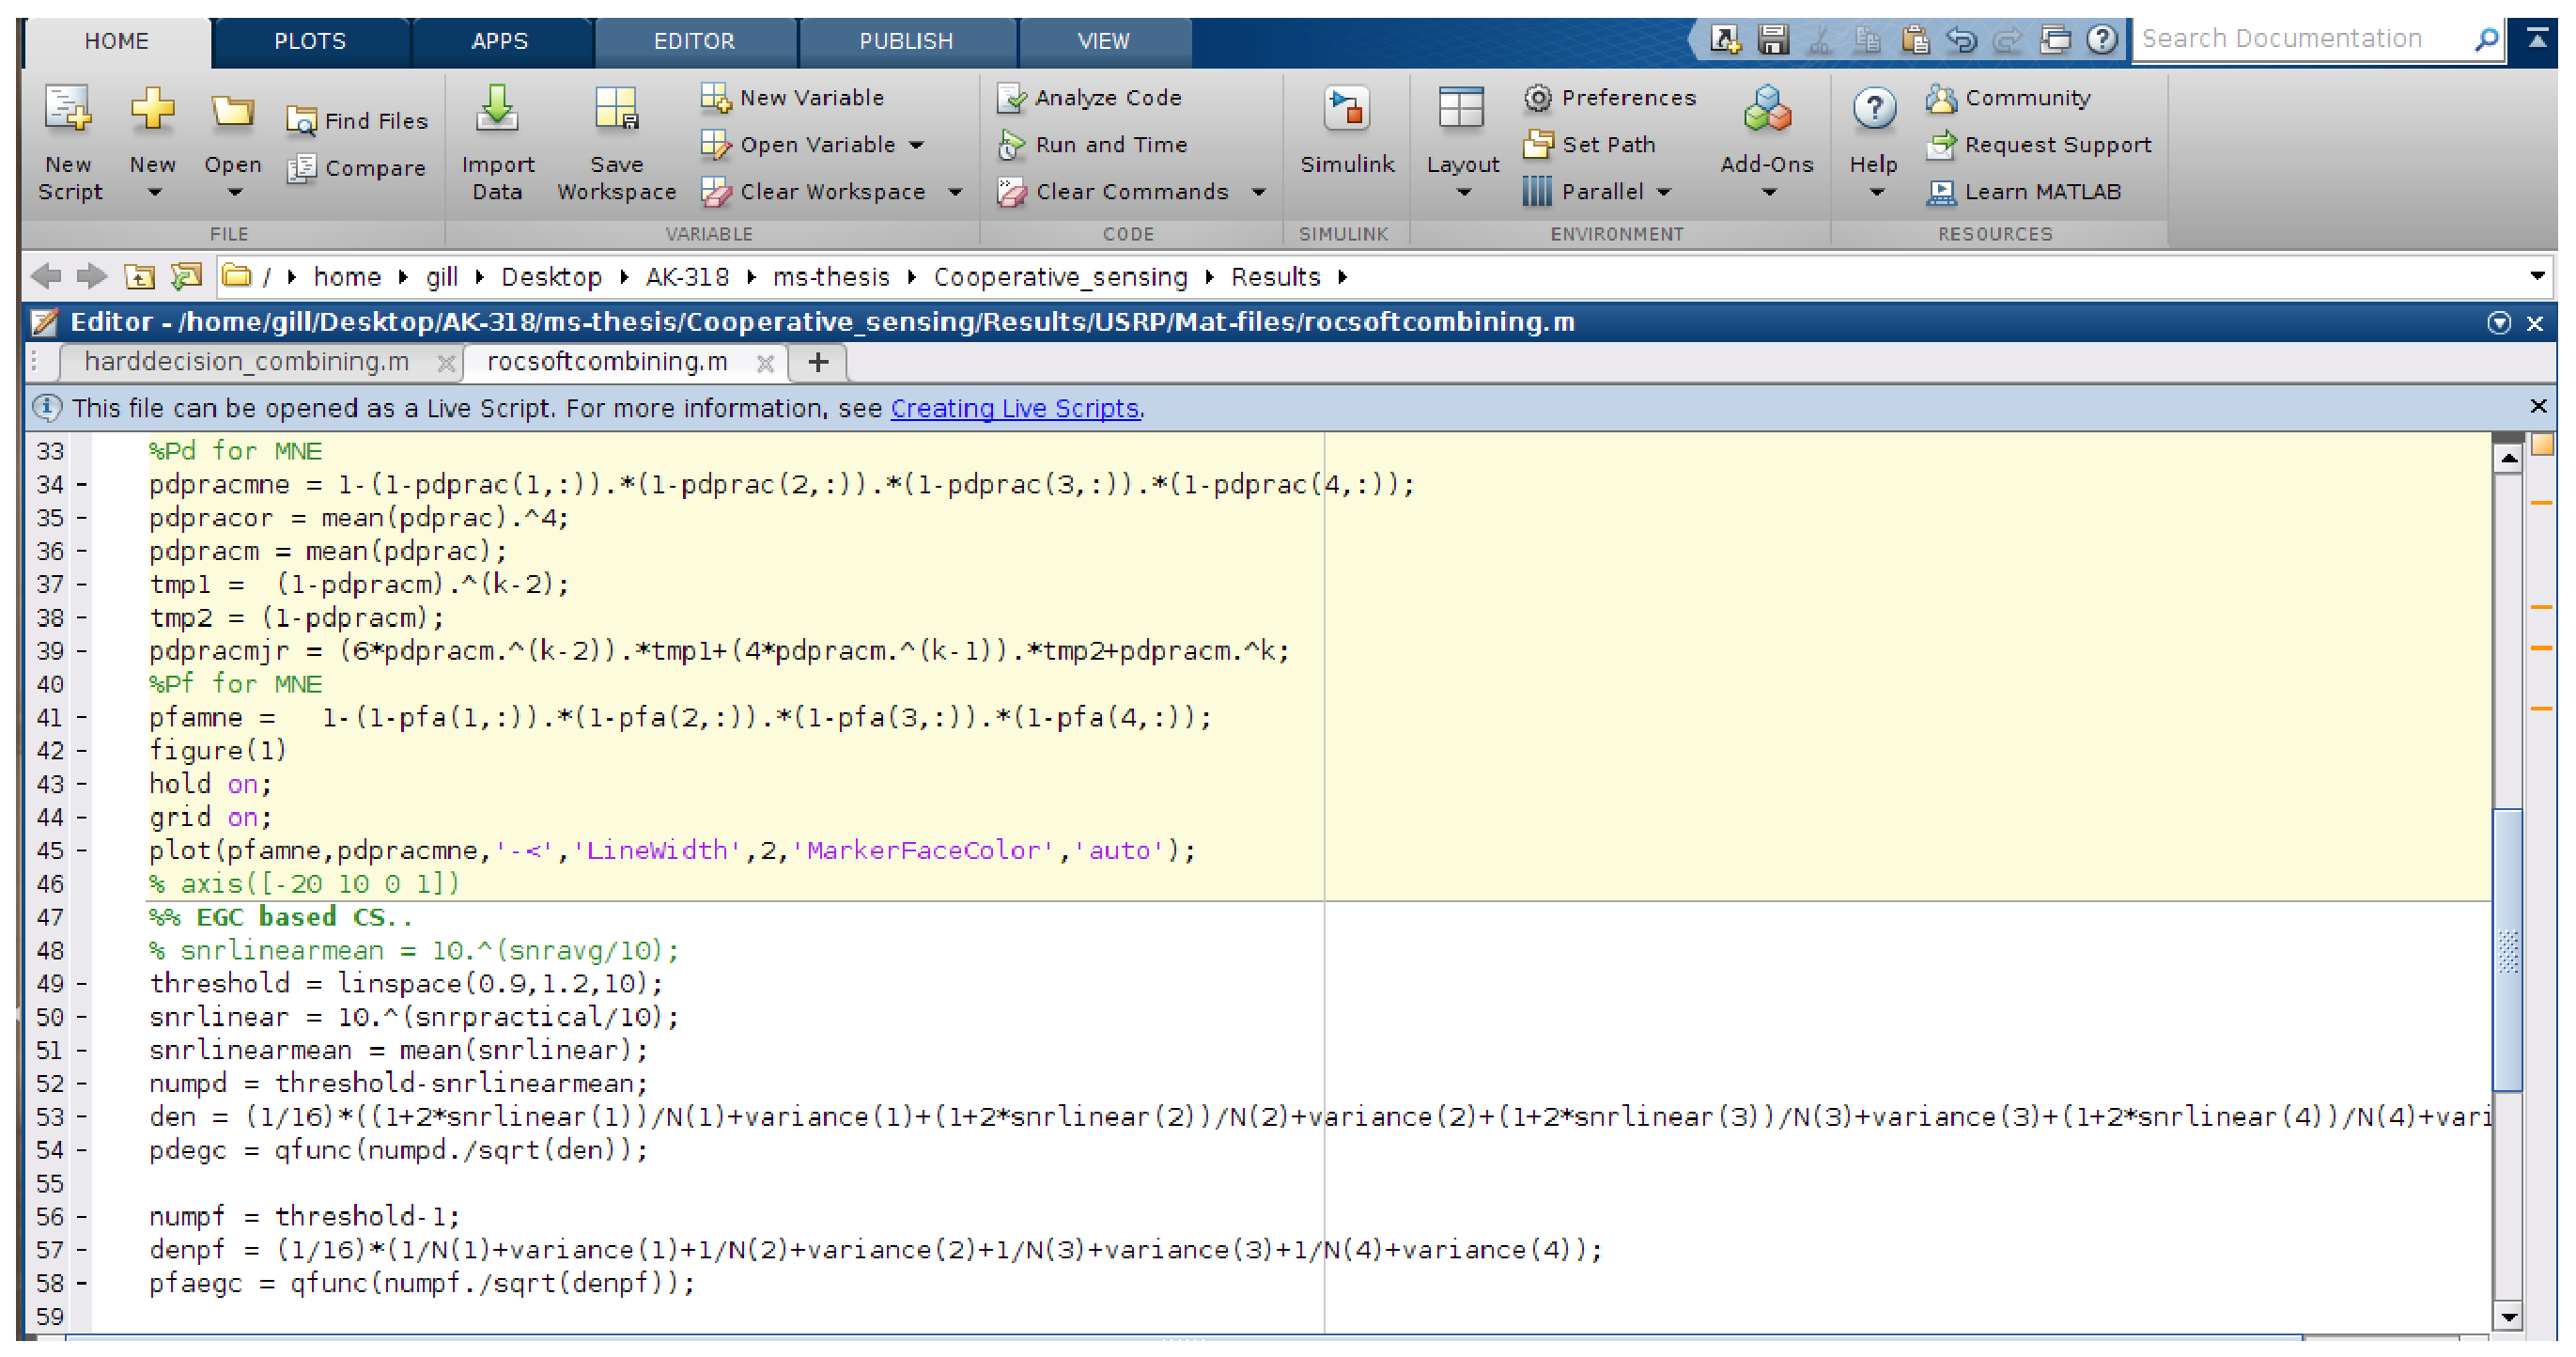
\includegraphics[width=\textwidth,keepaspectratio]{images/Gill/figs/matlab.eps}
    \caption{Screen capture of MATLAB editor running a code for computing receiver operating characteristics of soft decision combining scheme.}
\label{matlab}      
\end{figure}

MATLAB is an extremely well known engineering, mathematical, biological, and financial software suite. MATLAB provide massive data leverage and advanced communication system models and algorithm for significant data processing. In this thesis, we have used MATLAB for post-processing, where the results are later used in MATLAB which acts as a FC, and makes the decision based on the global test statistic for both hard and soft data fusion mechanism. Spectrum sensing data collected by the sensor nodes is dumped into static files, which are later processed in MATLAB to make decisions. Figure~\ref{matlab} shows the MATLAB editor where we computing the ROC characteristics of soft and hard decision combining schemes. The plots are also generated to compare both the schemes by data files collected in GNU Radio.

\section{Summary}
In this chapter, we discussed the heterogeneous cooperative spectrum sensing and examined various spectrum sensing techniques. We also discussed cognitive radios, CSS in heterogeneous networks, and software-defined radios in details. We discussed three popular spectrum sensing techniques and also describe the software-defined radios USRP N210 and RTL-SDR as well as their RF characteristics. Finally, we described the GNU Radio and MATLAB software tools used in the thesis to implement the proposed CSS test-bed. 
